% answers.tex —— 2010 年·普通高等学校招生考试·江苏卷 · 参考答案与详细解析片段
% 由 tools/generate_projects.py 依来源总账自 2010/2010_数学真题_江苏_试题.md + 2010/2010_数学真题_江苏_解析正文.md + 2010/2010_数学真题_江苏_答案要点.md 生成，勿手改（改源 MD 后重跑）

\begin{gktip}
固定候选 PDF 仅含题面，无答案页；以下解析与结论均由本库独立推导（非官方答案），并按 600 dpi 原页复核题面。原页未印分值，不补。
\end{gktip}

\begin{answer}
\gksolhead{1}{}

\textbf{题目}：

设集合 $A=\{-1,1,3\}$，$B=\{a+2,a^2+4\}$，$A\cap B=\{3\}$，则实数 $a=$ $\underline{\qquad}$。

\Needspace{4\baselineskip}
\textbf{解析}

\Needspace{5\baselineskip}
$A\cap B=\{3\}$，故 $3\in B$。由 $a^2+4\geqslant4$，只能

\nopagebreak[4]
\[a+2=3\iff a=1.\]

此时 $B=\{3,5\}$，$A\cap B=\{3\}$，符合。

\gkanswer{答案：$1$。}

\end{answer}
\begin{answer}
\gksolhead{2}{}

\textbf{题目}：

设复数 $z$ 满足 $z(2-3\mathrm i)=6+4\mathrm i$（其中 $\mathrm i$ 为虚数单位），则 $z$ 的模为$\underline{\qquad}$。

\Needspace{4\baselineskip}
\textbf{解析}

\nopagebreak[4]
\[z=\frac{6+4\mathrm i}{2-3\mathrm i}
=\frac{(6+4\mathrm i)(2+3\mathrm i)}{2^2+3^2}
=\frac{12+18\mathrm i+8\mathrm i-12}{13}
=2\mathrm i,\]

故 $|z|=2$。

\gkanswer{答案：$2$。}

\end{answer}
\begin{answer}
\gksolhead{3}{}

\textbf{题目}：

盒子中有大小相同的 $3$ 只白球，$1$ 只黑球，若从中随机地摸出两只球，则它们颜色不同的概率是$\underline{\qquad}$。

\Needspace{4\baselineskip}
\textbf{解析}

\Needspace{5\baselineskip}
从 $4$ 只球中取 $2$ 只共有 $\mathrm C_4^2=6$ 种。颜色不同即一白一黑，共 $3\times1=3$ 种，故概率为

\nopagebreak[4]
\[\frac36=\frac12.\]

\gkanswer{答案：$\dfrac12$。}

\end{answer}
\begin{answer}
\gksolhead{4}{}

\textbf{题目}：

某棉纺厂为了了解一批棉花的质量，从中随机抽取了 $100$ 根棉花纤维的长度（棉花纤维的长度是棉花质量的重要指标），所得数据都在区间 $[5,40]$ 中，其频率分布直方图如图所示，则其抽样的 $100$ 根中，有$\underline{\qquad}$根棉花纤维的长度小于 $20$ mm。
\nopagebreak[4]
\begin{center}% 2010 年江苏卷第 4 题：棉花纤维长度频率分布直方图。
% 来源 PDF：普通高考/2010/2010江苏.pdf，SHA-256 e701df878d51a700720549274fe7969bd54342f0f58acb051c516fc502b58af7。
% 原页：第 1 页（A3 三栏）第 1 栏中部，书页码 605。
% 重绘依据：组距 5，各组高度 0.01、0.01、0.04、0.05、0.06、0.02、0.01，样本 100。
\begin{tikzpicture}[semithick, x=0.32cm, y=60cm, every node/.style={inner sep=1.5pt, font=\small}]
  \draw[-stealth] (0,0) -- (41,0) node[right] {长度（mm）};
  \draw[-stealth] (0,0) -- (0,0.07) node[above] {$\dfrac{\text{频率}}{\text{组距}}$};
  \foreach \h/\lab in {0.01/0.01,0.02/0.02,0.04/0.04,0.05/0.05,0.06/0.06} {
    \draw (0,\h) -- (0.6,\h);
    \node[left,font=\scriptsize] at (-0.2,\h) {$\lab$};
  }
  \foreach \x/\h in {5/0.01,10/0.01,15/0.04,20/0.05,25/0.06,30/0.02,35/0.01} {
    \draw[fill=gray!25] (\x,0) rectangle (\x+5,\h);
  }
  \foreach \x in {0,5,10,15,20,25,30,35,40} {
    \draw (\x,0) -- (\x,-0.003) node[below] {$\x$};
  }
\end{tikzpicture}
\end{center}
\nopagebreak[4]
\Needspace{4\baselineskip}
\textbf{解析}

\Needspace{5\baselineskip}
长度小于 $20$ mm 的三组为 $[5,10)$、$[10,15)$、$[15,20)$，由直方图高度分别为 $0.01$、$0.01$、$0.04$，组距为 $5$。频数为

\nopagebreak[4]
\[100\times5\times(0.01+0.01+0.04)=100\times0.3=30.\]

\gkanswer{答案：$30$。}

\end{answer}
\begin{answer}
\gksolhead{5}{}

\textbf{题目}：

设函数 $f(x)=x(\mathrm e^x+a\mathrm e^{-x})$，$x\in\mathbf R$ 是偶函数，则实数 $a$ 的值为$\underline{\qquad}$。

\Needspace{4\baselineskip}
\textbf{解析}

\Needspace{5\baselineskip}
$f$ 为偶函数，$f(-x)=f(x)$：

\nopagebreak[4]
\[-x(\mathrm e^{-x}+a\mathrm e^x)=x(\mathrm e^x+a\mathrm e^{-x}).\]

\Needspace{5\baselineskip}
对任意 $x\neq0$ 比较系数：

\nopagebreak[4]
\[-1=a,\qquad -a=1,\]

故 $a=-1$。

\gkanswer{答案：$-1$。}

\end{answer}
\begin{answer}
\gksolhead{6}{}

\textbf{题目}：

在平面直角坐标系 $xOy$ 中，已知双曲线 $\dfrac{x^2}{4}-\dfrac{y^2}{12}=1$ 上一点 $M$ 的横坐标为 $3$，则点 $M$ 到此双曲线的右焦点的距离为$\underline{\qquad}$。

\Needspace{4\baselineskip}
\textbf{解析}

双曲线 $a=2$，$b^2=12$，$c=\sqrt{a^2+b^2}=4$，离心率 $e=2$。

\Needspace{5\baselineskip}
$M$ 在右支，$x_M=3>a$，到右焦点距离

\nopagebreak[4]
\[MF=ex_M-a=2\times3-2=4.\]

\gkanswer{答案：$4$。}

\end{answer}
\begin{answer}
\gksolhead{7}{}

\textbf{题目}：

如图是一个算法流程图，则输出 $S$ 的值是$\underline{\qquad}$。
\nopagebreak[4]
\begin{center}% 2010 年江苏卷第 7 题：算法流程图。
% 来源 PDF：普通高考/2010/2010江苏.pdf，SHA-256 e701df878d51a700720549274fe7969bd54342f0f58acb051c516fc502b58af7。
% 原页：第 1 页（A3 三栏）第 1 栏下部，书页码 605。
% 重绘依据：开始 → S←1 → n←1 → S←S+2^n → n←n+1 → 判断 S≥33；
%   否（右）→ 回到 S←S+2^n；是（下）→ 输出 S → 结束。
\begin{tikzpicture}[semithick, >=Stealth,
  every node/.style={inner sep=1.5pt, font=\small}]
  \node (start) [draw, rounded corners=4pt, minimum width=1.8cm, minimum height=0.55cm] at (0,0) {开始};
  \node (s1) [draw, minimum width=1.8cm, minimum height=0.6cm] at (0,-1.3) {$S\leftarrow1$};
  \node (n1) [draw, minimum width=1.8cm, minimum height=0.6cm] at (0,-2.65) {$n\leftarrow1$};
  \node (add) [draw, minimum width=3.0cm, minimum height=0.6cm] at (0,-4.15) {$S\leftarrow S+2^n$};
  \node (inc) [draw, minimum width=1.8cm, minimum height=0.6cm] at (0,-5.5) {$n\leftarrow n+1$};
  \node (test) [draw, diamond, aspect=2.2, minimum width=2.6cm, minimum height=1.1cm] at (0,-7.15) {$S\geqslant33$};
  \node (out) [draw, trapezium, trapezium left angle=72, trapezium right angle=108,
    minimum width=2.2cm, minimum height=0.55cm] at (0,-8.9) {输出 $S$};
  \node (end) [draw, rounded corners=4pt, minimum width=1.8cm, minimum height=0.55cm] at (0,-10.2) {结束};

  \draw[->] (start) -- (s1);
  \draw[->] (s1) -- (n1);
  \draw[->] (n1) -- (add);
  \draw[->] (add) -- (inc);
  \draw[->] (inc) -- (test);
  \draw[->] (test.south) -- node[right] {Y} (out.north);
  \draw[->] (out) -- (end);
  \draw[->] (test.east) -- node[above] {N} (4.2,-7.15) -- (4.2,-3.5) -- (0,-3.5) -- (add.north);
\end{tikzpicture}
\end{center}
\nopagebreak[4]
\Needspace{4\baselineskip}
\textbf{解析}

初始 $S=1$，$n=1$。循环执行 $S\leftarrow S+2^n$：

\begin{itemize}
\item $n=1$：$S=1+2=3$；
\item $n=2$：$S=3+4=7$；
\item $n=3$：$S=7+8=15$；
\item $n=4$：$S=15+16=31$；
\item $n=5$：$S=31+32=63$。
\end{itemize}

此时 $S=63\geqslant33$，输出 $63$。

\gkanswer{答案：$63$。}

\end{answer}
\begin{answer}
\gksolhead{8}{}

\textbf{题目}：

函数 $y=x^2$（$x>0$）的图象在点 $(a_k,a_k^2)$ 处的切线与 $x$ 轴交点的横坐标为 $a_{k+1}$，其中 $k\in\mathbf N^*$。若 $a_1=16$，则 $a_1+a_3+a_5$ 的值是$\underline{\qquad}$。

\Needspace{4\baselineskip}
\textbf{解析}

\Needspace{5\baselineskip}
$y=x^2$ 在 $(a_k,a_k^2)$ 处的切线斜率为 $2a_k$，切线为

\nopagebreak[4]
\[y-a_k^2=2a_k(x-a_k).\]

\Needspace{5\baselineskip}
令 $y=0$：

\nopagebreak[4]
\[-a_k^2=2a_k(x-a_k)\iff x=\frac{a_k}2.\]

\Needspace{5\baselineskip}
故 $a_{k+1}=\dfrac{a_k}2$，$\{a_k\}$ 为公比 $\dfrac12$ 的等比数列。$a_1=16$，

\nopagebreak[4]
\[a_3=4,\qquad a_5=1,\]

\nopagebreak[4]
\[a_1+a_3+a_5=16+4+1=21.\]

\gkanswer{答案：$21$。}

\end{answer}
\begin{answer}
\gksolhead{9}{}

\textbf{题目}：

在平面直角坐标系 $xOy$ 中，已知圆 $x^2+y^2=4$ 上有且仅有四个点到直线 $12x-5y+c=0$ 的距离为 $1$，则实数 $c$ 的取值范围是$\underline{\qquad}$。

\Needspace{4\baselineskip}
\textbf{解析}

\Needspace{5\baselineskip}
圆心到直线 $12x-5y+c=0$ 的距离

\nopagebreak[4]
\[d=\frac{|c|}{\sqrt{12^2+5^2}}=\frac{|c|}{13}.\]

\Needspace{5\baselineskip}
到该直线距离为 $1$ 的点的轨迹是两条平行线，它们到圆心的距离分别为 $d-1$ 与 $d+1$（取绝对值意义下）。圆半径为 $2$。要有且仅有四个交点，需两条平行线都与圆相交于两点：

\nopagebreak[4]
\[d+1<2\iff d<1,\qquad |d-1|<2\iff d<3.\]

\Needspace{5\baselineskip}
故 $d<1$，即

\nopagebreak[4]
\[\frac{|c|}{13}<1\iff -13<c<13.\]

\gkanswer{答案：$(-13,13)$。}

\end{answer}
\begin{answer}
\gksolhead{10}{}

\textbf{题目}：

定义在区间 $\left(0,\dfrac\pi2\right)$ 上的函数 $y=6\cos x$ 的图象与 $y=5\tan x$ 的图象的交于点 $P$，过点 $P$ 作 $x$ 轴的垂线，垂足为 $P_1$，直线 $PP_1$ 与 $y=\sin x$ 的图象交于点 $P_2$，则线段 $P_1P_2$ 的长为$\underline{\qquad}$。

\Needspace{4\baselineskip}
\textbf{解析}

\Needspace{5\baselineskip}
设交点 $P(x_0,y_0)$。由 $6\cos x_0=5\tan x_0$：

\nopagebreak[4]
\[6\cos^2x_0=5\sin x_0.\]

\Needspace{5\baselineskip}
令 $t=\sin x_0$，则 $6(1-t^2)=5t$：

\nopagebreak[4]
\[6t^2+5t-6=0\iff t=\frac23\ \text{\text{或}}\ -\frac32.\]

\Needspace{5\baselineskip}
因 $x_0\in\left(0,\dfrac\pi2\right)$，$t=\dfrac23$。$P_2$ 在 $y=\sin x$ 上且与 $P$ 横坐标相同，故 $P_2$ 的纵坐标为 $\dfrac23$，而 $P_1$ 在 $x$ 轴上，所以

\nopagebreak[4]
\[P_1P_2=\frac23.\]

\gkanswer{答案：$\dfrac23$。}

\end{answer}
\begin{answer}
\gksolhead{11}{}

\textbf{题目}：

已知函数 $f(x)=\begin{cases}x^2+1,&x\geqslant0,\\1,&x<0,\end{cases}$ 则满足不等式 $f(1-x^2)>f(2x)$ 的 $x$ 的取值范围是$\underline{\qquad}$。

\Needspace{4\baselineskip}
\textbf{解析}

由 $f(t)$ 的定义，$f(t)>1$ 当且仅当 $t>0$。

\Needspace{5\baselineskip}
令 $A=1-x^2$，$B=2x$，需 $A>0$，即

\nopagebreak[4]
\[-1<x<1.\]

\begin{itemize}
\item 若 $B\leqslant0$（即 $x\leqslant0$），$f(B)=1<f(A)$，成立；
\item 若 $B>0$（即 $x>0$），需 $A^2+1>B^2+1$，即
\end{itemize}

\nopagebreak[4]
\[1-x^2>2x\iff x^2+2x-1<0\iff x<\sqrt2-1.\]

\Needspace{5\baselineskip}
合并得

\nopagebreak[4]
\[-1<x<\sqrt2-1.\]

\gkanswer{答案：$(-1,\sqrt2-1)$。}

\end{answer}
\begin{answer}
\gksolhead{12}{}

\textbf{题目}：

设实数 $x,y$ 满足 $3\leqslant xy^2\leqslant8$，$4\leqslant\dfrac{x^2}{y}\leqslant9$，则 $\dfrac{x^3}{y^4}$ 的最大值是$\underline{\qquad}$。

\Needspace{4\baselineskip}
\textbf{解析}

\Needspace{5\baselineskip}
令 $u=xy^2$，$v=\dfrac{x^2}{y}$，则

\nopagebreak[4]
\[u^{-1}v^2=x^{-1}y^{-2}\cdot x^4y^{-2}=x^3y^{-4}=\frac{x^3}{y^4}.\]

\Needspace{5\baselineskip}
故

\nopagebreak[4]
\[\frac{x^3}{y^4}=\frac{v^2}{u}.\]

\Needspace{5\baselineskip}
由 $3\leqslant u\leqslant8$，$4\leqslant v\leqslant9$，

\nopagebreak[4]
\[\frac{x^3}{y^4}\leqslant\frac{9^2}{3}=27.\]

当 $u=3$，$v=9$ 时取到：解 $xy^2=3$，$\dfrac{x^2}{y}=9$ 得 $x=3$，$y=1$。故最大值为 $27$。

\gkanswer{答案：$27$。}

\end{answer}
\begin{answer}
\gksolhead{13}{}

\textbf{题目}：

在锐角 $\triangle ABC$ 中，角 $A$、$B$、$C$ 的对边分别为 $a$、$b$、$c$，若 $\dfrac ba+\dfrac ab=6\cos C$，则 $\dfrac{\tan C}{\tan A}+\dfrac{\tan C}{\tan B}$ 的值是$\underline{\qquad}$。

\Needspace{4\baselineskip}
\textbf{解析}

\Needspace{5\baselineskip}
由 $\dfrac ba+\dfrac ab=6\cos C$：

\nopagebreak[4]
\[\frac{a^2+b^2}{ab}=6\cos C\iff a^2+b^2=6ab\cos C.\]

\Needspace{5\baselineskip}
由余弦定理

\nopagebreak[4]
\[c^2=a^2+b^2-2ab\cos C=4ab\cos C.\]

\Needspace{5\baselineskip}
又

\nopagebreak[4]
\[\frac{\tan C}{\tan A}+\frac{\tan C}{\tan B}
=\tan C\left(\frac{\cos A}{\sin A}+\frac{\cos B}{\sin B}\right)
=\tan C\cdot\frac{\sin(A+B)}{\sin A\sin B}
=\frac{\sin^2C}{\cos C\sin A\sin B}.\]

\Needspace{5\baselineskip}
由正弦定理 $\sin A\sin B=\dfrac{ab}{4R^2}$，$\sin^2C=\dfrac{c^2}{4R^2}$，故

\nopagebreak[4]
\[\frac{\sin^2C}{\cos C\sin A\sin B}
=\frac{c^2}{ab\cos C}
=\frac{4ab\cos C}{ab\cos C}=4.\]

\gkanswer{答案：$4$。}

\end{answer}
\begin{answer}
\gksolhead{14}{}

\textbf{题目}：

\Needspace{5\baselineskip}
将边长为 $1$ m 的正三角形薄铁皮沿一条平行于某边的直线剪成两块，其中一块是梯形，记

\nopagebreak[4]
\[s=\frac{(\text{\text{梯形的周长}})^2}{\text{\text{梯形的面积}}},\]

则 $s$ 的最小值是$\underline{\qquad}$。

\Needspace{4\baselineskip}
\textbf{解析}

\Needspace{5\baselineskip}
设剪下的小正三角形边长为 $x$（$0<x<1$），则梯形两底为 $1$ 与 $x$，两腰均为 $1-x$，周长

\nopagebreak[4]
\[L=1+x+2(1-x)=3-x.\]

\Needspace{5\baselineskip}
梯形面积等于大三角形面积减去小三角形面积：

\nopagebreak[4]
\[S=\frac{\sqrt3}4(1-x^2).\]

\Needspace{5\baselineskip}
故

\nopagebreak[4]
\[s=\frac{(3-x)^2}{\frac{\sqrt3}4(1-x^2)}
=\frac{4(3-x)^2}{\sqrt3(1-x^2)}.\]

\Needspace{5\baselineskip}
令 $f(x)=\dfrac{(3-x)^2}{1-x^2}$。求导：

\nopagebreak[4]
\[f'(x)=\frac{-2(3-x)(1-x^2)+(3-x)^2\cdot2x}{(1-x^2)^2}
=\frac{2(3-x)(3x-1)}{(1-x^2)^2}.\]

\Needspace{5\baselineskip}
令 $f'(x)=0$ 得 $x=\dfrac13$，此时

\nopagebreak[4]
\[f\left(\frac13\right)=\frac{\left(\frac83\right)^2}{\frac89}=8.\]

\Needspace{5\baselineskip}
故

\nopagebreak[4]
\[s_{\min}=\frac{4\times8}{\sqrt3}=\frac{32\sqrt3}{3}.\]

\gkanswer{答案：$\dfrac{32\sqrt3}{3}$。}

\end{answer}
\begin{answer}
\gksolhead{15}{}

\textbf{题目}：

在平面直角坐标系 $xOy$ 中，已知点 $A(-1,-2)$、$B(2,3)$、$C(-2,-1)$。

（1）求以线段 $AB$、$AC$ 为邻边的平行四边形的两条对角线的长；

（2）设实数 $t$ 满足 $\left(\overrightarrow{AB}-t\overrightarrow{OC}\right)\cdot\overrightarrow{OC}=0$，求 $t$ 的值。

\Needspace{4\baselineskip}
\textbf{解析}

\Needspace{5\baselineskip}
（1）

\nopagebreak[4]
\[\overrightarrow{AB}=(3,5),\qquad \overrightarrow{AC}=(-1,1).\]

\Needspace{5\baselineskip}
两条对角线向量为

\nopagebreak[4]
\[\overrightarrow{AB}+\overrightarrow{AC}=(2,6),\]

\nopagebreak[4]
\[\overrightarrow{AB}-\overrightarrow{AC}=(4,4).\]

\Needspace{5\baselineskip}
长度分别为

\nopagebreak[4]
\[|(2,6)|=2\sqrt{10},\qquad |(4,4)|=4\sqrt2.\]

\Needspace{5\baselineskip}
（2）$\overrightarrow{OC}=(-2,-1)$，且

\nopagebreak[4]
\[\overrightarrow{AB}\cdot\overrightarrow{OC}=3\times(-2)+5\times(-1)=-11,\]

\nopagebreak[4]
\[|\overrightarrow{OC}|^2=5.\]

\Needspace{5\baselineskip}
由 $\left(\overrightarrow{AB}-t\overrightarrow{OC}\right)\cdot\overrightarrow{OC}=0$：

\nopagebreak[4]
\[-11-5t=0\iff t=-\frac{11}5.\]

\gkanswer{答案：（1）$2\sqrt{10}$，$4\sqrt2$；（2）$t=-\dfrac{11}5$。}

\end{answer}
\begin{answer}
\gksolhead{16}{}

\textbf{题目}：

如图，在四棱锥 $P-ABCD$ 中，$PD\perp$ 平面 $ABCD$，$PD=DC=BC=1$，$AB=2$，$AB\parallel DC$，$\angle BCD=90^\circ$。

（1）求证：$PC\perp BC$；

（2）求点 $A$ 到平面 $PBC$ 的距离。
\nopagebreak[4]
\begin{center}% 2010 年江苏卷第 16 题：四棱锥 P-ABCD。
% 来源 PDF：普通高考/2010/2010江苏.pdf，SHA-256 e701df878d51a700720549274fe7969bd54342f0f58acb051c516fc502b58af7。
% 原页：第 1 页（A3 三栏）第 3 栏下部，书页码 605。
% 重绘依据：D(0,0,0)、C(1,0,0)、B(1,1,0)、A(-1,1,0)、P(0,0,1)；
%   PD⊥底面，PD=DC=BC=1，AB=2，∠BCD=90°。PD 为高，画虚线。
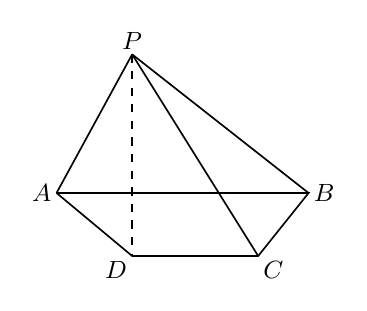
\begin{tikzpicture}[semithick, scale=1.6, every node/.style={inner sep=1.6pt, font=\small}]
  \coordinate (D) at (0,0);
  \coordinate (C) at (1,0);
  \coordinate (B) at (1.4,0.5);
  \coordinate (A) at (-0.6,0.5);
  \coordinate (P) at (0,1.6);

  \draw (A) -- (B) -- (C) -- (D) -- (A);
  \draw (P) -- (A);
  \draw (P) -- (B);
  \draw (P) -- (C);
  \draw[dashed] (P) -- (D);

  \node[below left] at (D) {$D$};
  \node[below right] at (C) {$C$};
  \node[right] at (B) {$B$};
  \node[left] at (A) {$A$};
  \node[above] at (P) {$P$};
\end{tikzpicture}
\end{center}
\nopagebreak[4]
\Needspace{4\baselineskip}
\textbf{解析}

\Needspace{5\baselineskip}
以 $D$ 为原点，$DC$ 为 $x$ 轴，$DP$ 为 $z$ 轴建立空间直角坐标系。由 $DC=BC=1$，$\angle BCD=90^\circ$，得

\nopagebreak[4]
\[D(0,0,0),\quad C(1,0,0),\quad B(1,1,0).\]

由 $PD=1$ 且 $PD\perp$ 平面 $ABCD$，$P(0,0,1)$。又 $AB\parallel DC$，$AB=2$，故 $A(-1,1,0)$。

\Needspace{5\baselineskip}
（1）

\nopagebreak[4]
\[\overrightarrow{PC}=(1,0,-1),\qquad \overrightarrow{BC}=(0,1,0),\]

\nopagebreak[4]
\[\overrightarrow{PC}\cdot\overrightarrow{BC}=0,\]

故 $PC\perp BC$。

\Needspace{5\baselineskip}
（2）平面 $PBC$ 中，

\nopagebreak[4]
\[\overrightarrow{PB}=(1,1,-1),\qquad \overrightarrow{PC}=(1,0,-1).\]

\Needspace{5\baselineskip}
法向量

\nopagebreak[4]
\[\boldsymbol n=\overrightarrow{PB}\times\overrightarrow{PC}
=(1,0,1).\]

\Needspace{5\baselineskip}
平面 $PBC$ 过 $C(1,0,0)$，方程为

\nopagebreak[4]
\[x+z-1=0.\]

\Needspace{5\baselineskip}
点 $A(-1,1,0)$ 到平面的距离

\nopagebreak[4]
\[d=\frac{|{-1}+0-1|}{\sqrt{1^2+0^2+1^2}}
=\frac2{\sqrt2}=\sqrt2.\]

\gkanswer{答案：（1）证明；（2）$\sqrt2$。}

\end{answer}
\begin{answer}
\gksolhead{17}{}

\textbf{题目}：

某兴趣小组测量电视塔 $AE$ 的高度 $H$（单位：m）。如示意图，垂直放置的标杆 $BC$ 的高度 $h=4$ m，仰角 $\angle ABE=\alpha$，$\angle ADE=\beta$。

（1）该小组已经测得一组 $\alpha$、$\beta$ 的值，算出了 $\tan\alpha=1.24$，$\tan\beta=1.20$，请据此算出 $H$ 的值；

（2）该小组分析若干测得的数据后，发现适当调整标杆到电视塔的距离 $d$（单位：m），使 $\alpha$ 与 $\beta$ 之差较大，可以提高测量精度。若电视塔实际高度为 $125$ m，试问 $d$ 为多少时，$\alpha-\beta$ 最大。
\nopagebreak[4]
\begin{center}% 2010 年江苏卷第 17 题：电视塔与标杆测高示意。
% 来源 PDF：普通高考/2010/2010江苏.pdf，SHA-256 e701df878d51a700720549274fe7969bd54342f0f58acb051c516fc502b58af7。
% 原页：第 1 页（A3 三栏）第 3 栏上部，书页码 605。
% 重绘依据：A 为塔底，AE 为塔高 H；B 为标杆底，BC=h；D 在 B 左侧；
%   ∠ABE=α，∠ADE=β；DB 与 AB=d 标注。
\begin{tikzpicture}[semithick, scale=1.0, every node/.style={inner sep=1.6pt, font=\small}]
  \coordinate (D) at (0,0);
  \coordinate (B) at (2.2,0);
  \coordinate (A) at (5.2,0);
  \coordinate (C) at (2.2,0.8);
  \coordinate (E) at (5.2,5);

  \draw (D) -- (A);
  \draw (A) -- (E);
  \draw (B) -- (C);
  \draw[dashed] (D) -- (E);
  \draw[dashed] (B) -- (E);

  \node[below] at (D) {$D$};
  \node[below] at (B) {$B$};
  \node[below] at (A) {$A$};
  \node[left] at (C) {$C$};
  \node[right] at (E) {$E$};
  \node[below] at (3.7,0) {$d$};
  \node at (1.3,0.35) {$\beta$};
  \node at (3.0,0.35) {$\alpha$};
\end{tikzpicture}
\end{center}
\nopagebreak[4]
\Needspace{4\baselineskip}
\textbf{解析}

\Needspace{5\baselineskip}
（1）设 $DB=x$。由标杆与电视塔平行，

\nopagebreak[4]
\[\frac hH=\frac{x}{d+x}.\]

\Needspace{5\baselineskip}
又

\nopagebreak[4]
\[\tan\beta=\frac H{d+x}\iff d+x=\frac H{\tan\beta}=\frac H{1.20},\]

\Needspace{5\baselineskip}
故

\nopagebreak[4]
\[x=DB=\frac h{\tan\beta}=\frac4{1.20}=\frac{10}3.\]

\Needspace{5\baselineskip}
由 $d=\dfrac H{\tan\alpha}=\dfrac H{1.24}$，代入 $\dfrac hH=\dfrac x{d+x}$：

\nopagebreak[4]
\[H=\frac{h(d+x)}x
\iff Hx=h(d+x)=h\left(\frac H{1.24}+x\right).\]

\Needspace{5\baselineskip}
整理：

\nopagebreak[4]
\[H\left(x-\frac h{1.24}\right)=hx
\iff H=\frac{hx}{x-\frac h{1.24}}.\]

\Needspace{5\baselineskip}
代入 $h=4$，$x=\dfrac{10}3$：

\nopagebreak[4]
\[H=\frac{4\times\frac{10}3}{\frac{10}3-\frac4{1.24}}=124.\]

\Needspace{5\baselineskip}
（2）一般地，由（1）的思路可得

\nopagebreak[4]
\[\tan\alpha=\frac Hd,\qquad \tan\beta=\frac{H-h}{d}.\]

\Needspace{5\baselineskip}
于是

\nopagebreak[4]
\[\tan(\alpha-\beta)
=\frac{\tan\alpha-\tan\beta}{1+\tan\alpha\tan\beta}
=\frac{\frac hd}{1+\frac{H(H-h)}{d^2}}
=\frac{hd}{d^2+H(H-h)}.\]

\Needspace{5\baselineskip}
由基本不等式

\nopagebreak[4]
\[d^2+H(H-h)\geqslant2d\sqrt{H(H-h)},\]

\Needspace{5\baselineskip}
故

\nopagebreak[4]
\[\tan(\alpha-\beta)\leqslant\frac{hd}{2d\sqrt{H(H-h)}}
=\frac h{2\sqrt{H(H-h)}},\]

等号当 $d=\sqrt{H(H-h)}$ 时成立。

\Needspace{5\baselineskip}
代入 $H=125$，$h=4$：

\nopagebreak[4]
\[d=\sqrt{125\times121}=55\sqrt5.\]

\gkanswer{答案：（1）$H=124$；（2）$d=55\sqrt5$。}

\end{answer}
\begin{answer}
\gksolhead{18}{}

\textbf{题目}：

在平面直角坐标系 $xOy$ 中，如图，已知椭圆 $\dfrac{x^2}{9}+\dfrac{y^2}{5}=1$ 的左、右顶点为 $A$、$B$，右焦点为 $F$。设过点 $T(t,m)$ 的直线 $TA$、$TB$ 与此椭圆分别交于点 $M(x_1,y_1)$、$N(x_2,y_2)$，其中 $m>0$，$y_1>0$，$y_2<0$。

（1）设动点 $P$ 满足 $PF^2-PB^2=4$，求点 $P$ 的轨迹；

（2）设 $x_1=2$，$x_2=\dfrac13$，求点 $T$ 的坐标；

（3）设 $t=9$，求证：直线 $MN$ 必过 $x$ 轴上的一定点（其坐标与 $m$ 无关）。
\nopagebreak[4]
\begin{center}% 2010 年江苏卷第 18 题：椭圆与直线 TA、TB。
% 来源 PDF：普通高考/2010/2010江苏.pdf，SHA-256 e701df878d51a700720549274fe7969bd54342f0f58acb051c516fc502b58af7。
% 原页：第 1 页（A3 三栏）第 3 栏下部，书页码 605。
% 重绘依据：椭圆 x^2/9+y^2/5=1，A(-3,0)、B(3,0)、F(2,0)；
%   T(9,m) 在右上方，TA 交椭圆于 M，TB 交椭圆于 N。
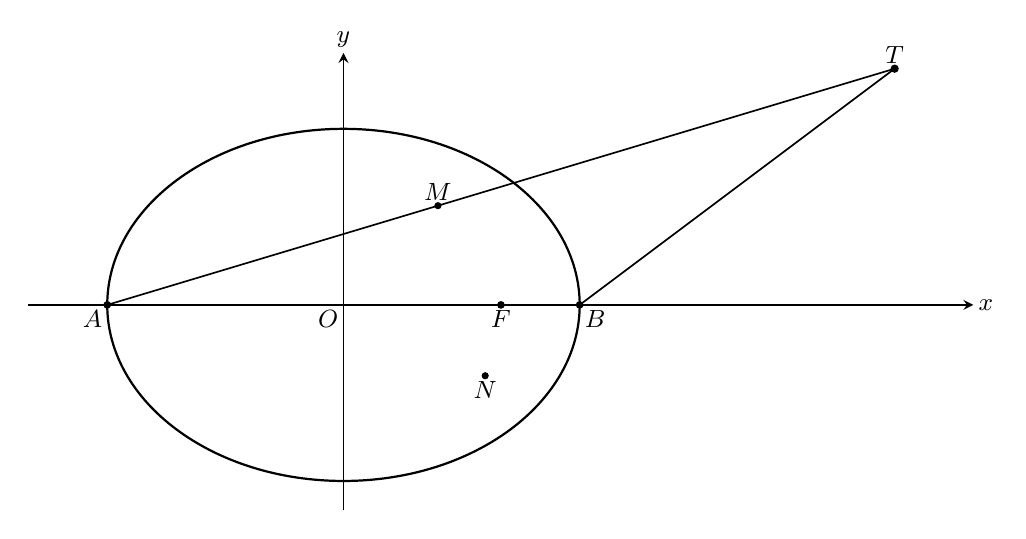
\begin{tikzpicture}[semithick, scale=1.0, every node/.style={inner sep=1.6pt, font=\small}]
  \draw[-stealth] (-4,0) -- (8,0) node[right] {$x$};
  \draw[-stealth] (0,-2.6) -- (0,3.2) node[above] {$y$};
  \draw[thick] (0,0) ellipse (3 and 2.236);
  \fill (-3,0) circle (1.4pt) node[below left] {$A$};
  \fill (3,0) circle (1.4pt) node[below right] {$B$};
  \fill (2,0) circle (1.4pt) node[below] {$F$};
  \fill (7,3) circle (1.5pt) node[above] {$T$};
  \draw (7,3) -- (-3,0);
  \draw (7,3) -- (3,0);
  \fill (1.2,1.26) circle (1.3pt) node[above] {$M$};
  \fill (1.8,-0.9) circle (1.3pt) node[below] {$N$};
  \node[below left] at (0,0) {$O$};
\end{tikzpicture}
\end{center}
\nopagebreak[4]
\Needspace{4\baselineskip}
\textbf{解析}

\Needspace{5\baselineskip}
（1）$A(-3,0)$，$B(3,0)$，$F(2,0)$。设 $P(x,y)$，

\nopagebreak[4]
\[PF^2-PB^2=4\]

\Needspace{5\baselineskip}
即

\nopagebreak[4]
\[(x-2)^2+y^2-\left[(x-3)^2+y^2\right]=4.\]

\Needspace{5\baselineskip}
化简：

\nopagebreak[4]
\[(x^2-4x+4)-(x^2-6x+9)=4
\iff 2x-5=4
\iff x=\frac92.\]

故轨迹为直线 $x=\dfrac92$。

\Needspace{5\baselineskip}
（2）$x_1=2$ 时，

\nopagebreak[4]
\[\frac49+\frac{y_1^2}5=1\iff y_1^2=\frac{25}9,\]

由 $y_1>0$ 得 $y_1=\dfrac53$。

\Needspace{5\baselineskip}
$x_2=\dfrac13$ 时，

\nopagebreak[4]
\[\frac1{81}+\frac{y_2^2}5=1\iff y_2^2=\frac{400}{81},\]

由 $y_2<0$ 得 $y_2=-\dfrac{20}9$。

\Needspace{5\baselineskip}
直线 $AM$：

\nopagebreak[4]
\[M\left(2,\frac53\right),\quad A(-3,0)
\implies y=\frac13(x+3).\]

\Needspace{5\baselineskip}
直线 $BN$：

\nopagebreak[4]
\[N\left(\frac13,-\frac{20}9\right),\quad B(3,0)
\implies y=\frac56(x-3).\]

\Needspace{5\baselineskip}
联立：

\nopagebreak[4]
\[\frac13(x+3)=\frac56(x-3)
\iff 2(x+3)=5(x-3)
\iff x=7.\]

\Needspace{5\baselineskip}
代回 $y=\dfrac{10}3$，故

\nopagebreak[4]
\[T\left(7,\frac{10}3\right).\]

（3）$t=9$，$T(9,m)$。

\Needspace{5\baselineskip}
直线 $TA$：$y=k(x+3)$，$k=\dfrac m{12}$。代入椭圆 $5x^2+9y^2=45$：

\nopagebreak[4]
\[(5+9k^2)x^2+54k^2x+81k^2-45=0.\]

\Needspace{5\baselineskip}
一根为 $x=-3$，故另一根

\nopagebreak[4]
\[x_1=\frac{3(5-9k^2)}{5+9k^2}.\]

\Needspace{5\baselineskip}
于是

\nopagebreak[4]
\[y_1=k(x_1+3)=\frac{30k}{5+9k^2}.\]

\Needspace{5\baselineskip}
直线 $TB$：$y=k_2(x-3)$，$k_2=\dfrac m6=2k$。同理

\nopagebreak[4]
\[x_2=\frac{3(9k_2^2-5)}{5+9k_2^2},\qquad
y_2=-\frac{30k_2}{5+9k_2^2}.\]

\Needspace{5\baselineskip}
要证 $MN$ 过 $(1,0)$，只需证

\nopagebreak[4]
\[\frac{y_1}{x_1-1}=\frac{y_2}{x_2-1}.\]

\Needspace{5\baselineskip}
计算：

\nopagebreak[4]
\[x_1-1=\frac{3(5-9k^2)-(5+9k^2)}{5+9k^2}
=\frac{10-36k^2}{5+9k^2},\]

\nopagebreak[4]
\[\frac{y_1}{x_1-1}
=\frac{30k}{10-36k^2}
=\frac{15k}{5-18k^2}.\]

\Needspace{5\baselineskip}
又 $k_2=2k$：

\nopagebreak[4]
\[x_2-1=\frac{3(36k^2-5)-(5+36k^2)}{5+36k^2}
=\frac{72k^2-20}{5+36k^2},\]

\nopagebreak[4]
\[\frac{y_2}{x_2-1}
=\frac{-60k}{72k^2-20}
=\frac{15k}{5-18k^2}.\]

\Needspace{5\baselineskip}
两者相等，故 $M$、$N$、$(1,0)$ 三点共线。即直线 $MN$ 恒过定点

\nopagebreak[4]
\[(1,0).\]

\gkanswer{答案：（1）$x=\dfrac92$；（2）$T\left(7,\dfrac{10}3\right)$；（3）定点 $(1,0)$。}

\end{answer}
\begin{answer}
\gksolhead{19}{}

\textbf{题目}：

设各项均为正数的数列 $\{a_n\}$ 的前 $n$ 项和为 $S_n$。已知 $2a_2=a_1+a_3$，数列 $\{\sqrt{S_n}\}$ 是公差为 $d$ 的等差数列。

（1）求数列 $\{a_n\}$ 的通项公式（用 $n,d$ 表示）；

（2）设 $c$ 为实数，对满足 $m+n=3k$ 且 $m\neq n$ 的任意正整数 $m,n,k$，不等式 $S_m+S_n>cS_k$ 都成立。求证：$c$ 的最大值为 $\dfrac92$。

\Needspace{4\baselineskip}
\textbf{解析}

\Needspace{5\baselineskip}
（1）设 $\sqrt{S_n}=b_1+(n-1)d$，则

\nopagebreak[4]
\[S_n=[b_1+(n-1)d]^2.\]

\Needspace{5\baselineskip}
由 $a_1=S_1=b_1^2$，

\nopagebreak[4]
\[a_2=S_2-S_1=2b_1d+d^2,\]

\nopagebreak[4]
\[a_3=S_3-S_2=2b_1d+3d^2.\]

\Needspace{5\baselineskip}
代入 $2a_2=a_1+a_3$：

\nopagebreak[4]
\[4b_1d+2d^2=b_1^2+2b_1d+3d^2,\]

\Needspace{5\baselineskip}
整理得

\nopagebreak[4]
\[b_1^2-2b_1d+d^2=0\iff (b_1-d)^2=0,\]

\Needspace{5\baselineskip}
故 $b_1=d$，$S_n=n^2d^2$。于是

\nopagebreak[4]
\[a_n=S_n-S_{n-1}=n^2d^2-(n-1)^2d^2=(2n-1)d^2.\]

\Needspace{5\baselineskip}
（2）由（1），$S_m+S_n=(m^2+n^2)d^2$，$S_k=k^2d^2$。不等式化为

\nopagebreak[4]
\[m^2+n^2>c k^2.\]

\Needspace{5\baselineskip}
令

\nopagebreak[4]
\[m=\frac{3k}2+s,\qquad n=\frac{3k}2-s,\]

\Needspace{5\baselineskip}
其中 $s\neq0$。则

\nopagebreak[4]
\[m^2+n^2=\frac{9k^2}2+2s^2.\]

\Needspace{5\baselineskip}
故

\nopagebreak[4]
\[\frac{m^2+n^2}{k^2}=\frac92+\frac{2s^2}{k^2}>\frac92.\]

因此 $c=\dfrac92$ 时不等式恒成立。

\Needspace{5\baselineskip}
若 $c>\dfrac92$，取 $k$ 为偶数、$s=1$，则

\nopagebreak[4]
\[\frac{m^2+n^2}{k^2}=\frac92+\frac2{k^2}<c\]

当 $k$ 充分大时成立，此时 $S_m+S_n<cS_k$，不等式不成立。

\Needspace{5\baselineskip}
故 $c$ 的最大值为

\nopagebreak[4]
\[\frac92.\]

\gkanswer{答案：（1）$a_n=(2n-1)d^2$；（2）证明，$c_{\max}=\dfrac92$。}

\end{answer}
\begin{answer}
\gksolhead{20}{}

\textbf{题目}：

设 $f(x)$ 是定义在区间 $(1,+\infty)$ 上的函数，其导函数为 $f'(x)$。如果存在实数 $a$ 和函数 $h(x)$，其中 $h(x)$ 对任意的 $x\in(1,+\infty)$ 都有 $h(x)>0$，使得 $f'(x)=h(x)(x^2-ax+1)$，则称函数 $f(x)$ 具有性质 $P(a)$。

（1）设函数 $f(x)=\ln x+\dfrac{b+2}{x+1}$（$x>1$），其中 $b$ 为实数。

① 求证：函数 $f(x)$ 具有性质 $P(b)$；

② 求函数 $f(x)$ 的单调区间。

（2）已知函数 $g(x)$ 具有性质 $P(2)$，给定 $x_1,x_2\in(1,+\infty)$，$x_1<x_2$，设 $m$ 为实数，$\alpha=mx_1+(1-m)x_2$，$\beta=(1-m)x_1+mx_2$，且 $\alpha>1$，$\beta>1$。若 $|g(\alpha)-g(\beta)|<|g(x_1)-g(x_2)|$，求 $m$ 的取值范围。

\Needspace{4\baselineskip}
\textbf{解析}

\Needspace{5\baselineskip}
（1）①

\nopagebreak[4]
\[f'(x)=\frac1x-\frac{b+2}{(x+1)^2}
=\frac{(x+1)^2-(b+2)x}{x(x+1)^2}
=\frac{x^2-bx+1}{x(x+1)^2}.\]

\Needspace{5\baselineskip}
取

\nopagebreak[4]
\[h(x)=\frac1{x(x+1)^2}>0\quad(x>1),\]

则 $f'(x)=h(x)(x^2-bx+1)$，故 $f(x)$ 具有性质 $P(b)$。

② $x^2-bx+1$ 的判别式 $\Delta=b^2-4$。

当 $b\leqslant2$ 时，$\Delta\leqslant0$，且二次项系数为正，故 $x^2-bx+1\geqslant0$ 在 $(1,+\infty)$ 上恒成立，$f'(x)\geqslant0$，$f$ 在 $(1,+\infty)$ 上递增。

\Needspace{5\baselineskip}
当 $b>2$ 时，两根为

\nopagebreak[4]
\[r_{1,2}=\frac{b\pm\sqrt{b^2-4}}2,\qquad r_1<1<r_2.\]

故 $f$ 在 $(1,r_2)$ 上递减，在 $(r_2,+\infty)$ 上递增。

\Needspace{5\baselineskip}
（2）$g$ 具有性质 $P(2)$，故

\nopagebreak[4]
\[g'(x)=h(x)(x^2-2x+1)=h(x)(x-1)^2\geqslant0,\]

$g$ 在 $(1,+\infty)$ 上递增。

由 $x_1<x_2$：

\begin{itemize}
\item 若 $0<m<1$，则 $\alpha,\beta$ 均为 $x_1,x_2$ 的严格凸组合，故 $\alpha,\beta\in(x_1,x_2)$（或 $\alpha=\beta$）。于是
\end{itemize}

\nopagebreak[4]
\[|g(\alpha)-g(\beta)|<g(x_2)-g(x_1)=|g(x_1)-g(x_2)|.\]

\begin{itemize}
\item 若 $m\leqslant0$ 或 $m\geqslant1$，则 $\alpha,\beta$ 中至少一个不在 $(x_1,x_2)$ 内，$|g(\alpha)-g(\beta)|\geqslant g(x_2)-g(x_1)$，不满足。
\end{itemize}

\Needspace{5\baselineskip}
故

\nopagebreak[4]
\[0<m<1.\]

\gkanswer{答案：（1）① 证明；② $b\leqslant2$ 时在 $(1,+\infty)$ 递增；$b>2$ 时在 $\left(1,\dfrac{b+\sqrt{b^2-4}}2\right)$ 递减，在 $\left(\dfrac{b+\sqrt{b^2-4}}2,+\infty\right)$ 递增；（2）$0<m<1$。}

\end{answer}
\begin{answer}
\gksolhead{21}{}

\textbf{题目}：

四选二。

【A】如图，$AB$ 是 $\odot O$ 的直径，$D$ 为 $\odot O$ 上一点，过点 $D$ 作 $\odot O$ 的切线交 $AB$ 延长线于点 $C$。若 $DA=DC$，求证：$AB=2BC$。
\nopagebreak[4]
\begin{center}% 2010 年江苏卷第 21A 题：圆 O 的切线与直径。
% 来源 PDF：普通高考/2010/2010江苏.pdf，SHA-256 e701df878d51a700720549274fe7969bd54342f0f58acb051c516fc502b58af7。
% 原页：第 2 页（A3 三栏）第 1 栏上部，书页码 606。
% 重绘依据：AB 为直径，D 在圆上，切线 DC 交 AB 延长线于 C；DA=DC。
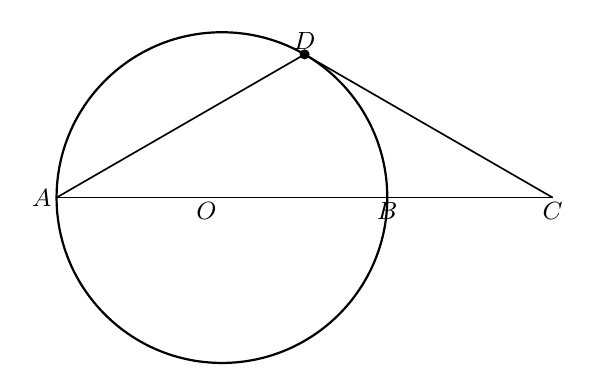
\begin{tikzpicture}[semithick, scale=1.4, every node/.style={inner sep=1.6pt, font=\small}]
  \draw[thick] (0,0) circle (1.5);
  \coordinate (O) at (0,0);
  \coordinate (A) at (-1.5,0);
  \coordinate (B) at (1.5,0);
  \coordinate (C) at (3,0);
  \coordinate (D) at (0.75,1.299);

  \draw (A) -- (C);
  \draw (D) -- (C);
  \draw (A) -- (D);
  \fill (D) circle (1.3pt);
  \node[left] at (A) {$A$};
  \node[below] at (B) {$B$};
  \node[below] at (C) {$C$};
  \node[above] at (D) {$D$};
  \node[below left] at (O) {$O$};
\end{tikzpicture}
\end{center}
\nopagebreak[4]
【B】在平面直角坐标系 $xOy$ 中，$A(0,0)$，$B(-2,0)$，$C(-2,1)$，设 $k$ 为非零实数。矩阵 $M=\begin{bmatrix}k&0\\0&1\end{bmatrix}$，$N=\begin{bmatrix}0&1\\1&0\end{bmatrix}$，点 $A$、$B$、$C$ 在矩阵 $MN$ 对应的变换下得到的点分别为 $A_1$、$B_1$、$C_1$，$\triangle A_1B_1C_1$ 的面积是 $\triangle ABC$ 面积的 $2$ 倍，求实数 $k$ 的值。

【C】在极坐标系中，圆 $\rho=2\cos\theta$ 与直线 $3\rho\cos\theta+4\rho\sin\theta+a=0$ 相切，求实数 $a$ 的值。

【D】设 $a,b$ 是非负实数，求证：$a^3+b^3\geqslant\sqrt{ab}(a^2+b^2)$。

\Needspace{4\baselineskip}
\textbf{解析}

【A】设圆半径为 $r$，$O$ 为原点，$A(-r,0)$，$B(r,0)$，$C(r+x,0)$，其中 $x=BC$。

\Needspace{5\baselineskip}
设 $D(u,v)$。由 $D$ 在圆上且在 $C$ 处的切线上，切点横坐标满足

\nopagebreak[4]
\[u=\frac{r^2}{r+x}.\]

\Needspace{5\baselineskip}
又 $DA=DC$：

\nopagebreak[4]
\[(u+r)^2+v^2=(r+x-u)^2+v^2
\iff u+r=r+x-u
\iff u=\frac x2.\]

\Needspace{5\baselineskip}
故

\nopagebreak[4]
\[\frac{r^2}{r+x}=\frac x2
\iff 2r^2=xr+x^2
\iff (x-r)(x+2r)=0.\]

\Needspace{5\baselineskip}
因 $x>0$，故 $x=r$，即

\nopagebreak[4]
\[BC=r=\frac{AB}2\iff AB=2BC.\]

\Needspace{5\baselineskip}
【B】$MN=\begin{bmatrix}0&k\\1&0\end{bmatrix}$，对应变换

\nopagebreak[4]
\[(x,y)\mapsto(ky,x).\]

\Needspace{5\baselineskip}
故

\nopagebreak[4]
\[A_1(0,0),\quad B_1(0,-2),\quad C_1(k,-2).\]

\Needspace{5\baselineskip}
$\triangle A_1B_1C_1$ 的面积为

\nopagebreak[4]
\[\frac12\cdot|k|\cdot2=|k|.\]

\Needspace{5\baselineskip}
原 $\triangle ABC$ 的面积为 $1$。由题意 $|k|=2$，故

\nopagebreak[4]
\[k=\pm2.\]

\Needspace{5\baselineskip}
【C】$\rho=2\cos\theta$ 化为

\nopagebreak[4]
\[x^2+y^2=2x\iff (x-1)^2+y^2=1,\]

\Needspace{5\baselineskip}
圆心 $(1,0)$，半径 $1$。直线 $3x+4y+a=0$ 与圆相切：

\nopagebreak[4]
\[\frac{|3+a|}{\sqrt{3^2+4^2}}=1
\iff |a+3|=5,\]

\Needspace{5\baselineskip}
故

\nopagebreak[4]
\[a=2\ \text{\text{或}}\ a=-8.\]

\Needspace{5\baselineskip}
【D】若 $a=0$ 或 $b=0$，不等式显然成立。设 $a,b>0$，令 $t=\sqrt{\dfrac ab}>0$，则 $a=t^2b$。原不等式两边除以 $b^2$：

\nopagebreak[4]
\[t^5+\frac1t\geqslant t^4+1.\]

\Needspace{5\baselineskip}
等价于

\nopagebreak[4]
\[t^6+1\geqslant t^5+t
\iff (t-1)(t^5-1)\geqslant0,\]

对 $t>0$ 恒成立。故原不等式成立，等号当且仅当 $a=b$。

\gkanswer{答案：A 证明；B $k=\pm2$；C $a=2$ 或 $-8$；D 证明。}

\end{answer}
\begin{answer}
\gksolhead{22}{}

\textbf{题目}：

某工厂生产甲、乙两种产品。甲产品的一等品率为 $80\%$，二等品率为 $20\%$；乙产品的一等品率为 $90\%$，二等品率为 $10\%$。生产 $1$ 件甲产品，若是一等品则获得利润 $4$ 万元，若是二等品则亏损 $1$ 万元；生产 $1$ 件乙产品，若是一等品则获得利润 $6$ 万元，若是二等品则亏损 $2$ 万元。设生产各种产品相互独立。

（1）记 $X$（单位：万元）为生产 $1$ 件甲产品和 $1$ 件乙产品可获得的总利润，求 $X$ 的分布列；

（2）求生产 $4$ 件甲产品所获得的利润不少于 $10$ 万元的概率。

\Needspace{4\baselineskip}
\textbf{解析}

（1）$X$ 的取值及概率：

\begin{itemize}
\item 甲、乙均为一等品：$X=4+6=10$，
\end{itemize}

\nopagebreak[4]
\[P=0.8\times0.9=0.72;\]

\begin{itemize}
\item 甲一等、乙二等：$X=4-2=2$，
\end{itemize}

\nopagebreak[4]
\[P=0.8\times0.1=0.08;\]

\begin{itemize}
\item 甲二等、乙一等：$X=-1+6=5$，
\end{itemize}

\nopagebreak[4]
\[P=0.2\times0.9=0.18;\]

\begin{itemize}
\item 甲、乙均为二等品：$X=-1-2=-3$，
\end{itemize}

\nopagebreak[4]
\[P=0.2\times0.1=0.02.\]

分布列：

\begin{center}
\begin{tabular}{lllll}
\toprule
$X$ & $-3$ & $2$ & $5$ & $10$ \\
\midrule
$P$ & $0.02$ & $0.08$ & $0.18$ & $0.72$ \\
\bottomrule
\end{tabular}
\end{center}

\Needspace{5\baselineskip}
（2）设 $4$ 件甲产品中一等品有 $k$ 件，利润为

\nopagebreak[4]
\[4k-(4-k)=5k-4.\]

\Needspace{5\baselineskip}
要求

\nopagebreak[4]
\[5k-4\geqslant10\iff k\geqslant\frac{14}5,\]

\Needspace{5\baselineskip}
故 $k=3$ 或 $4$。概率为

\nopagebreak[4]
\[\mathrm C_4^3(0.8)^3(0.2)+(0.8)^4
=4\times0.512\times0.2+0.4096
=0.4096+0.4096=0.8192=\frac{512}{625}.\]

\gkanswer{答案：（1）分布列见下；（2）$\dfrac{512}{625}$。}

\end{answer}
\begin{answer}
\gksolhead{23}{}

\textbf{题目}：

已知 $\triangle ABC$ 的三边长都是有理数。

（1）求证：$\cos A$ 是有理数；

（2）求证：对任意正整数 $n$，$\cos nA$ 是有理数。

\Needspace{4\baselineskip}
\textbf{解析}

\Needspace{5\baselineskip}
（1）设三边 $a,b,c$ 均为有理数。由余弦定理

\nopagebreak[4]
\[\cos A=\frac{b^2+c^2-a^2}{2bc}.\]

有理数对四则运算封闭，故 $\cos A$ 为有理数。

（2）对 $n$ 归纳证明。

\Needspace{5\baselineskip}
$n=1$ 时 $\cos A$ 有理；$n=2$ 时

\nopagebreak[4]
\[\cos2A=2\cos^2A-1\]

有理。

\Needspace{5\baselineskip}
设 $\cos kA$ 与 $\cos(k-1)A$ 均为有理数。由积化和差公式

\nopagebreak[4]
\[\cos(k+1)A=2\cos A\cos kA-\cos(k-1)A,\]

右边为有理数，故 $\cos(k+1)A$ 也为有理数。

由数学归纳法，对任意正整数 $n$，$\cos nA$ 是有理数。

\gkanswer{答案：（1）证明；（2）证明。}

\end{answer}